\documentclass[11pt,a4paper]{article}
\usepackage[utf8]{inputenc}
\usepackage[T1]{fontenc}
\usepackage[a4paper,margin=1in]{geometry}
\usepackage{amsmath,amssymb}
\usepackage{booktabs}
\usepackage{tabularx}
\usepackage{array}
\usepackage{longtable}
\usepackage{graphicx}
\usepackage{float}
\usepackage{caption}
\usepackage{xcolor}
\usepackage{enumitem}
\usepackage{fancyhdr}
\usepackage{tikz}
\usetikzlibrary{shapes.geometric,arrows.meta,positioning,fit,backgrounds,calc}
\usepackage[hidelinks]{hyperref}

\definecolor{accent}{HTML}{1F4E79}
\definecolor{soft}{HTML}{F2F4F7}
\definecolor{rule}{HTML}{B9C2CC}
\definecolor{ok}{HTML}{2E7D32}
\definecolor{bad}{HTML}{B3261E}

\pagestyle{fancy}
\fancyhf{}
\renewcommand{\headrulewidth}{0.4pt}
\fancyhead[L]{\small\itshape ThinkStack}
\fancyhead[R]{\small\itshape \leftmark}
\fancyfoot[C]{\small\thepage}

\setlist{itemsep=2pt, topsep=4pt}

\newcommand{\coverpage}[2]{%
\begin{titlepage}
\centering
{\large CHRIST (Deemed to be University), Bengaluru\par}
{\large Department of Computer Science\par}
\vspace{1.1cm}
{\Large\bfseries #1\par}
\vspace{0.35cm}
{\large Course: CSC481-5, Computer Science Project\par}
{\large Semester V\par}
\vspace{1.5cm}
{\Huge\bfseries ThinkStack\par}
\vspace{0.35cm}
{\large\itshape #2\par}
\vspace{1.5cm}
{\large\bfseries Submitted by\par}
\vspace{0.3cm}
\begin{tabular}{clc}
\toprule
\textbf{Sl. No.} & \textbf{Student Name} & \textbf{Register No.} \\
\midrule
1. & Aditya Mehta & 2440204 \\
2. & Jitvan Chadha & 2440222 \\
3. & Ritesh K R & 2440233 \\
\bottomrule
\end{tabular}
\vspace{1.2cm}

\begin{tabular}{ll}
\textbf{Guide:} & Dr. New Begin \\
\textbf{Class:} & 5BSC CS \\
\textbf{Repository:} & \texttt{github.com/get-thinkstack/ThinkStack} \\
\end{tabular}
\vfill
{\large July 2026\par}
\end{titlepage}
}

\newcommand{\evidence}[1]{%
\begin{center}
\fcolorbox{rule}{soft}{\parbox{0.93\linewidth}{\small #1}}
\end{center}}

\newcommand{\yes}{\textcolor{ok}{\textbf{Yes}}}
\newcommand{\no}{\textcolor{bad}{\textbf{No}}}

\begin{document}
\coverpage{Sprint I: Design and Development Document}{Offline SLM-Based Research Assistant}

\tableofcontents
\newpage

\section{Sprint Overview}
\markboth{Sprint Overview}{}

\subsection{Period and scope}

Sprint I ran from 5 June 2026 to 24 June 2026. Its objective was to establish a
working research assistant in which every core capability functioned end to end
with local inference: ingesting research papers, retrieving from them,
summarising them, conversing about them, protecting them, and drafting LaTeX.

\begin{center}
\small
\begin{tabular}{@{}ll@{}}
\toprule
\textbf{Attribute} & \textbf{Value} \\
\midrule
Duration & 5 June 2026 to 24 June 2026 \\
Active development days & 11 \\
Commits & 29 \\
Deliverable & a functional application running from source \\
\bottomrule
\end{tabular}
\end{center}

The team of three worked jointly across the sprint, with responsibilities
rotating between backend services, interface work, and the desktop shell. Work
was integrated through pull requests into a shared branch.

\subsection{Sprint goal statement}

\evidence{\textbf{Goal.} A user should be able to add a PDF to the application,
ask a question about it, receive an answer drawn from that document rather than
from the model's memory, and draft a LaTeX section with assistance, with all
computation performed on the local machine and no network dependency.}

\section{Requirements Addressed}

\subsection{Functional requirements}

\begin{center}
\small
\begin{tabularx}{\linewidth}{@{}llX@{}}
\toprule
\textbf{ID} & \textbf{Requirement} & \textbf{Realisation in Sprint I} \\
\midrule
FR-1 & Ingest PDF documents & extraction, metadata recovery, chunking, embedding, storage \\
FR-2 & Search the collection & dense semantic retrieval combined with keyword retrieval \\
FR-3 & Summarise a document & structured summarisation through the local model \\
FR-4 & Extract key claims & claim extraction returning structured output \\
FR-5 & Cluster themes & thematic grouping across the corpus \\
FR-6 & Identify research gaps & gap analysis with suggestion generation \\
FR-7 & Converse about papers & retrieval-grounded chat over selected documents \\
FR-8 & Protect sensitive papers & password-based encryption with authenticated ciphertext \\
FR-9 & Draft LaTeX & AI-assisted editor with local compilation to PDF \\
\bottomrule
\end{tabularx}
\end{center}

\subsection{Non-functional requirements}

\begin{itemize}[leftmargin=*]
  \item \textbf{Privacy.} No document, prompt, or derived artefact may leave the
        machine. This is the defining constraint of the product and it
        eliminated every hosted-inference design.
  \item \textbf{Offline operation.} The application must function with the
        network disconnected.
  \item \textbf{Commodity hardware.} The target is an ordinary student laptop,
        assumed to have 8 to 16 GB of memory and no usable GPU.
  \item \textbf{No running cost.} No API keys and no subscription.
\end{itemize}

\section{System Design}

\subsection{Architectural style}

A layered architecture was adopted, with a REST interface between the user
interface and the domain logic.

\begin{figure}[H]
\centering
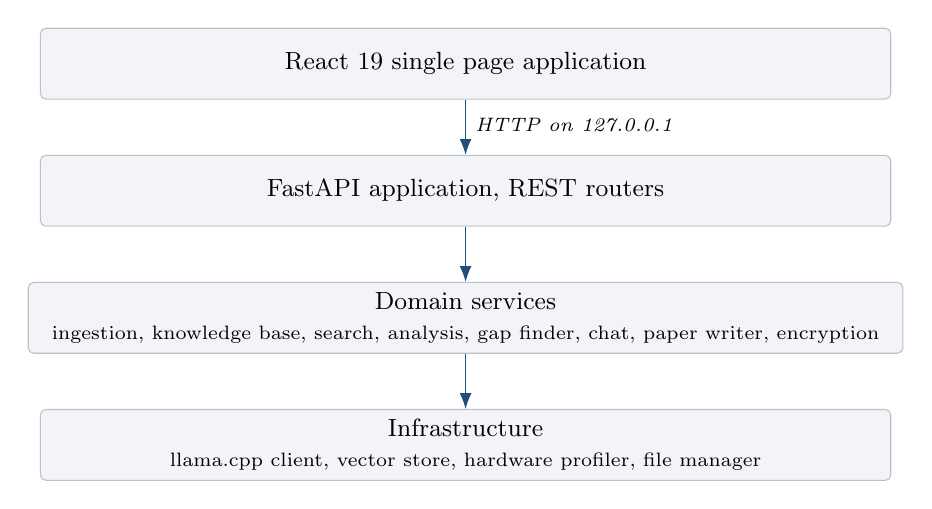
\begin{tikzpicture}[
  node distance=7mm,
  box/.style={draw=rule, fill=soft, rounded corners=2pt, minimum height=9mm,
              inner xsep=3mm, align=center, font=\small},
  arr/.style={-{Latex[length=2mm]}, draw=accent}
]
\node[box, minimum width=108mm] (ui) {React 19 single page application};
\node[box, minimum width=108mm, below=of ui] (api) {FastAPI application, REST routers};
\node[box, minimum width=108mm, below=of api] (dom) {Domain services\\
  \scriptsize ingestion, knowledge base, search, analysis, gap finder, chat, paper writer, encryption};
\node[box, minimum width=108mm, below=of dom] (inf) {Infrastructure\\
  \scriptsize llama.cpp client, vector store, hardware profiler, file manager};
\draw[arr] (ui) -- node[right,font=\scriptsize\itshape]{HTTP on 127.0.0.1} (api);
\draw[arr] (api) -- (dom);
\draw[arr] (dom) -- (inf);
\end{tikzpicture}
\caption{Layered architecture established in Sprint I.}
\end{figure}

\paragraph{Design rationale.} A local HTTP boundary was chosen over embedding
the Python runtime directly into the desktop shell. Three properties followed
from that decision: the same backend serves both a desktop window and an
ordinary browser without duplicated code; a failure inside the model runtime
terminates a supervised child process rather than the whole application; and the
interface between layers is inspectable with ordinary HTTP tooling, which later
made automated validation of the packaged product possible.

\subsection{Ingestion pipeline design}

\begin{figure}[H]
\centering
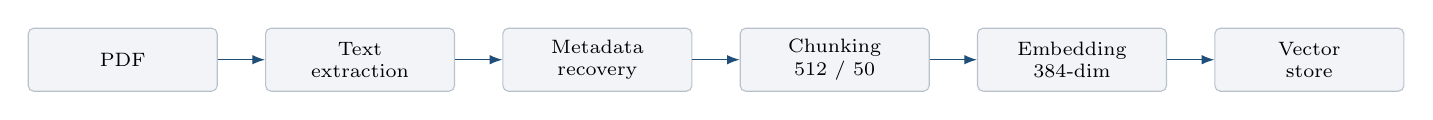
\begin{tikzpicture}[
  node distance=6mm,
  st/.style={draw=rule, fill=soft, rounded corners=2pt, minimum height=8mm,
             minimum width=24mm, align=center, font=\scriptsize},
  arr/.style={-{Latex[length=1.6mm]}, draw=accent}
]
\node[st] (a) {PDF};
\node[st, right=of a] (b) {Text\\extraction};
\node[st, right=of b] (c) {Metadata\\recovery};
\node[st, right=of c] (d) {Chunking\\512 / 50};
\node[st, right=of d] (e) {Embedding\\384-dim};
\node[st, right=of e] (f) {Vector\\store};
\foreach \i/\j in {a/b,b/c,c/d,d/e,e/f} \draw[arr] (\i) -- (\j);
\end{tikzpicture}
\caption{Document ingestion. Chunks are 512 tokens with 50 tokens of overlap.}
\end{figure}

\paragraph{Chunking strategy.} Text is divided by a descending hierarchy of
separators: paragraph breaks first, then line breaks, then sentence boundaries,
then words. This preserves semantic units, so a retrieved chunk is more likely
to be independently meaningful. Overlap of 50 tokens ensures that a statement
spanning a boundary is not lost to both neighbours.

\paragraph{Metadata recovery.} Regular expressions extract title, authors,
abstract and year. The local model is invoked only when that leaves the title or
abstract empty, so an expensive inference call is avoided for well-formed
papers.

\subsection{Retrieval design}

Two retrieval methods are computed and fused rather than one being chosen:

\begin{itemize}[leftmargin=*]
  \item \textbf{Dense retrieval} embeds the query into the same 384-dimensional
        space as the chunks and ranks by cosine similarity. This finds
        paraphrase, where the query and the document share meaning but no words.
  \item \textbf{Keyword retrieval} scores by BM25. This finds exact technical
        terms, identifiers and notation, where dense retrieval is weak.
  \item \textbf{Reciprocal rank fusion} combines the two ranked lists, rewarding
        documents that both methods rank highly without requiring the two score
        scales to be comparable.
\end{itemize}

\subsection{Storage design}

A file-based vector store using NumPy cosine similarity was chosen over an
embedded database. The reasoning was the governing constraint: a database
engine is another component that must install correctly on a machine the
developers cannot inspect. The accepted cost is that the keyword index is
rebuilt per query, which is acceptable for a personal library and is recorded as
a known limitation.

\subsection{Encryption design}

\begin{center}
\small
\begin{tabular}{@{}ll@{}}
\toprule
\textbf{Concern} & \textbf{Mechanism} \\
\midrule
Key derivation & Argon2id, memory-hard, resistant to hardware brute force \\
Confidentiality and integrity & AES-256-GCM, authenticated encryption \\
Format & versioned envelope, so the scheme can change without data loss \\
\bottomrule
\end{tabular}
\end{center}

Authenticated encryption was chosen deliberately over an unauthenticated mode:
tampering with a stored paper is detected at decryption rather than producing
plausible but corrupted output.

\subsection{Paper writer design}

The paper writer accepts a natural language description and returns compilable
LaTeX produced by the local model. The compiler was designed to be forgiving,
because a language model of this size produces markup that is frequently almost
correct:

\begin{itemize}[leftmargin=*]
  \item missing package declarations are inserted automatically;
  \item a bare fragment is wrapped into a complete document;
  \item compilation continues past recoverable errors, and the existence of a
        PDF is treated as success with errors surfaced as warnings;
  \item when a pass produces no PDF, the failing environment is progressively
        neutralised and compilation retried, so a single malformed figure does
        not cost the author the entire document.
\end{itemize}

\section{Implementation}

\subsection{Technology selected}

\begin{center}
\small
\begin{tabular}{@{}lll@{}}
\toprule
\textbf{Concern} & \textbf{Choice} & \textbf{Reason} \\
\midrule
Backend & FastAPI, Uvicorn & typed request models, automatic API schema \\
Interface & React 19, Vite & component model suited to distinct feature panes \\
Desktop shell & Tauri 2, Rust & small binary, uses the system webview \\
Inference & llama.cpp, GGUF & runs quantised models on CPU \\
Embeddings & all-MiniLM-L6-v2 & 384 dimensions, small enough to bundle \\
Keyword search & rank\_bm25 & no service to install \\
PDF handling & PyMuPDF, pdfplumber & PyMuPDF for speed, pdfplumber as fallback \\
Encryption & argon2-cffi, cryptography & standard, audited implementations \\
\bottomrule
\end{tabular}
\end{center}

\subsection{Model selection}

Qwen2.5 instruction models were selected at 0.5 and 1.5 billion parameters,
quantised to four bits in the \texttt{Q4\_K\_M} scheme. The 0.5B model is used
for conversational tasks where latency is visible to the user, and the 1.5B
model for tasks that must emit structured output. Quantisation is what makes
CPU execution viable within the memory of an ordinary laptop.

\subsection{Work completed}

\begin{center}
\small
\begin{tabularx}{\linewidth}{@{}lX@{}}
\toprule
\textbf{Date} & \textbf{Outcome} \\
\midrule
5 to 10 June & repository established, initial documentation, first working demonstration \\
11 to 16 June & interface iteration, project naming corrected in documentation \\
17 June & project renamed from ScholarLens to ThinkStack; backend audit and correction; architecture decision log and feature reference established \\
17 June & chat assistant verified against the local runtime \\
19 to 20 June & desktop application initialised with Tauri; first DevOps scripts \\
20 to 21 June & encryption and decryption implemented; interface refinements; edge cases in the encryption flow corrected \\
23 June & LaTeX editor and auto-healing compiler implemented \\
24 June & interface unified with the LaTeX editor; desktop packaging configured; security design documented \\
\bottomrule
\end{tabularx}
\end{center}

\section{Testing Performed}

Testing in Sprint I was manual and feature-directed. Each capability was
exercised through the interface against real research papers: a document was
ingested, searched, summarised, discussed through chat, encrypted and
decrypted, and a LaTeX section was drafted and compiled.

No automated test suite existed at the end of Sprint I. This is stated plainly
because it became the central weakness addressed in Sprint II.

\section{Sprint I Outcome}

\begin{center}
\small
\begin{tabular}{@{}lc@{}}
\toprule
\textbf{Objective} & \textbf{Achieved} \\
\midrule
Ingest and index PDF documents & \yes \\
Hybrid semantic and keyword retrieval & \yes \\
Summarisation, claim extraction, thematic clustering & \yes \\
Research gap identification & \yes \\
Retrieval-grounded chat & \yes \\
Local document encryption & \yes \\
AI-assisted LaTeX editor with compilation & \yes \\
Desktop shell around the application & \yes \\
Runs with the network disconnected & \yes \\
\midrule
Installable by a user on an unprepared machine & \no \\
Automated regression testing & \no \\
\bottomrule
\end{tabular}
\end{center}

\subsection{Retrospective}

\paragraph{What succeeded.} Every technically demanding component was completed
within the sprint. Local inference with acceptable latency, hybrid retrieval,
authenticated encryption and a fault-tolerant LaTeX compiler all worked.
Recording architectural decisions as they were taken, beginning on 17 June,
produced a written rationale that proved valuable in the following sprint.

\paragraph{What was deferred.} The application ran from a source checkout on
machines that already had Python, a model runtime and a LaTeX distribution
installed. Nothing had been packaged, distributed, or executed anywhere else.
The distinction between software that works and software that has been shown to
work on another machine was not yet appreciated, and defined the entire second
sprint.

\paragraph{Carried into Sprint II.}

\begin{enumerate}[leftmargin=*]
  \item Package the application into installers for Linux, macOS and Windows.
  \item Remove every assumption that the user's machine resembles a developer's.
  \item Introduce automated testing.
  \item Establish a repeatable release process.
\end{enumerate}

\end{document}
